\chapter{Analysis}
\label{chap:analysis}
% recap of introduction - motiovation, goals + related work
% brief intorduction of the purpose of chapter
After framing context of the platform by presenting both motivation and goals with previewing related solutions, we take a closer look at the overall analysis for our software.
The purpose is to present the requirements placed on the system, primarily determined by the standard ordering process in the eCommerce sector.
In addition, the requirements resulting from the planned test deployment will be presented as well as the definition of the specific requirements that will guide the development of the platform. %The purpose is to present and understand the order dispatch process flow and the practical implications of implementing and testing this solution within a real-world company environment.
This analysis is the foundation for a solution that not only meets technical specifications but also addresses practical business needs within a logistics sector and day-to-day usage.

This chapter will begin with a necessary introduction to the order dispatch process \ref{sec:order-dispatching-process}. 
Understanding this process is necessary to frame the context in which the entire system operates and in which users operate.
Then, after understanding the context, in the \ref{sec:real-world-applicability} section, an approach to testing the system will be presented, both from both the integration and user perspective.
Finally, after defining the environment in which the system is set and a way to verify the functionality, we can go to the \ref{sec:requirements} section.
This section will present the functional and non-functional requirements on the system.

% 



\section{Order dispatching process}
\label{sec:order-dispatching-process}
% describe how orders are processed from ordering online, to SAP Draft objects, to SAP order objects to packing list to finally passing to the shipping company and printing label with consignment list
This section dives into the general life-cycle of an order from the moment it is placed to the final delivery.
We will take into account the most simple and straightforward approach, which is usually the starting point for many companies and warehouses.
Defining this process helps to understand weaknesses and identify opportunities for automation and efficiency improvements.
Suppose a customer of a company is shopping in an e-Commerce store:

\begin{figure}[H]\centering
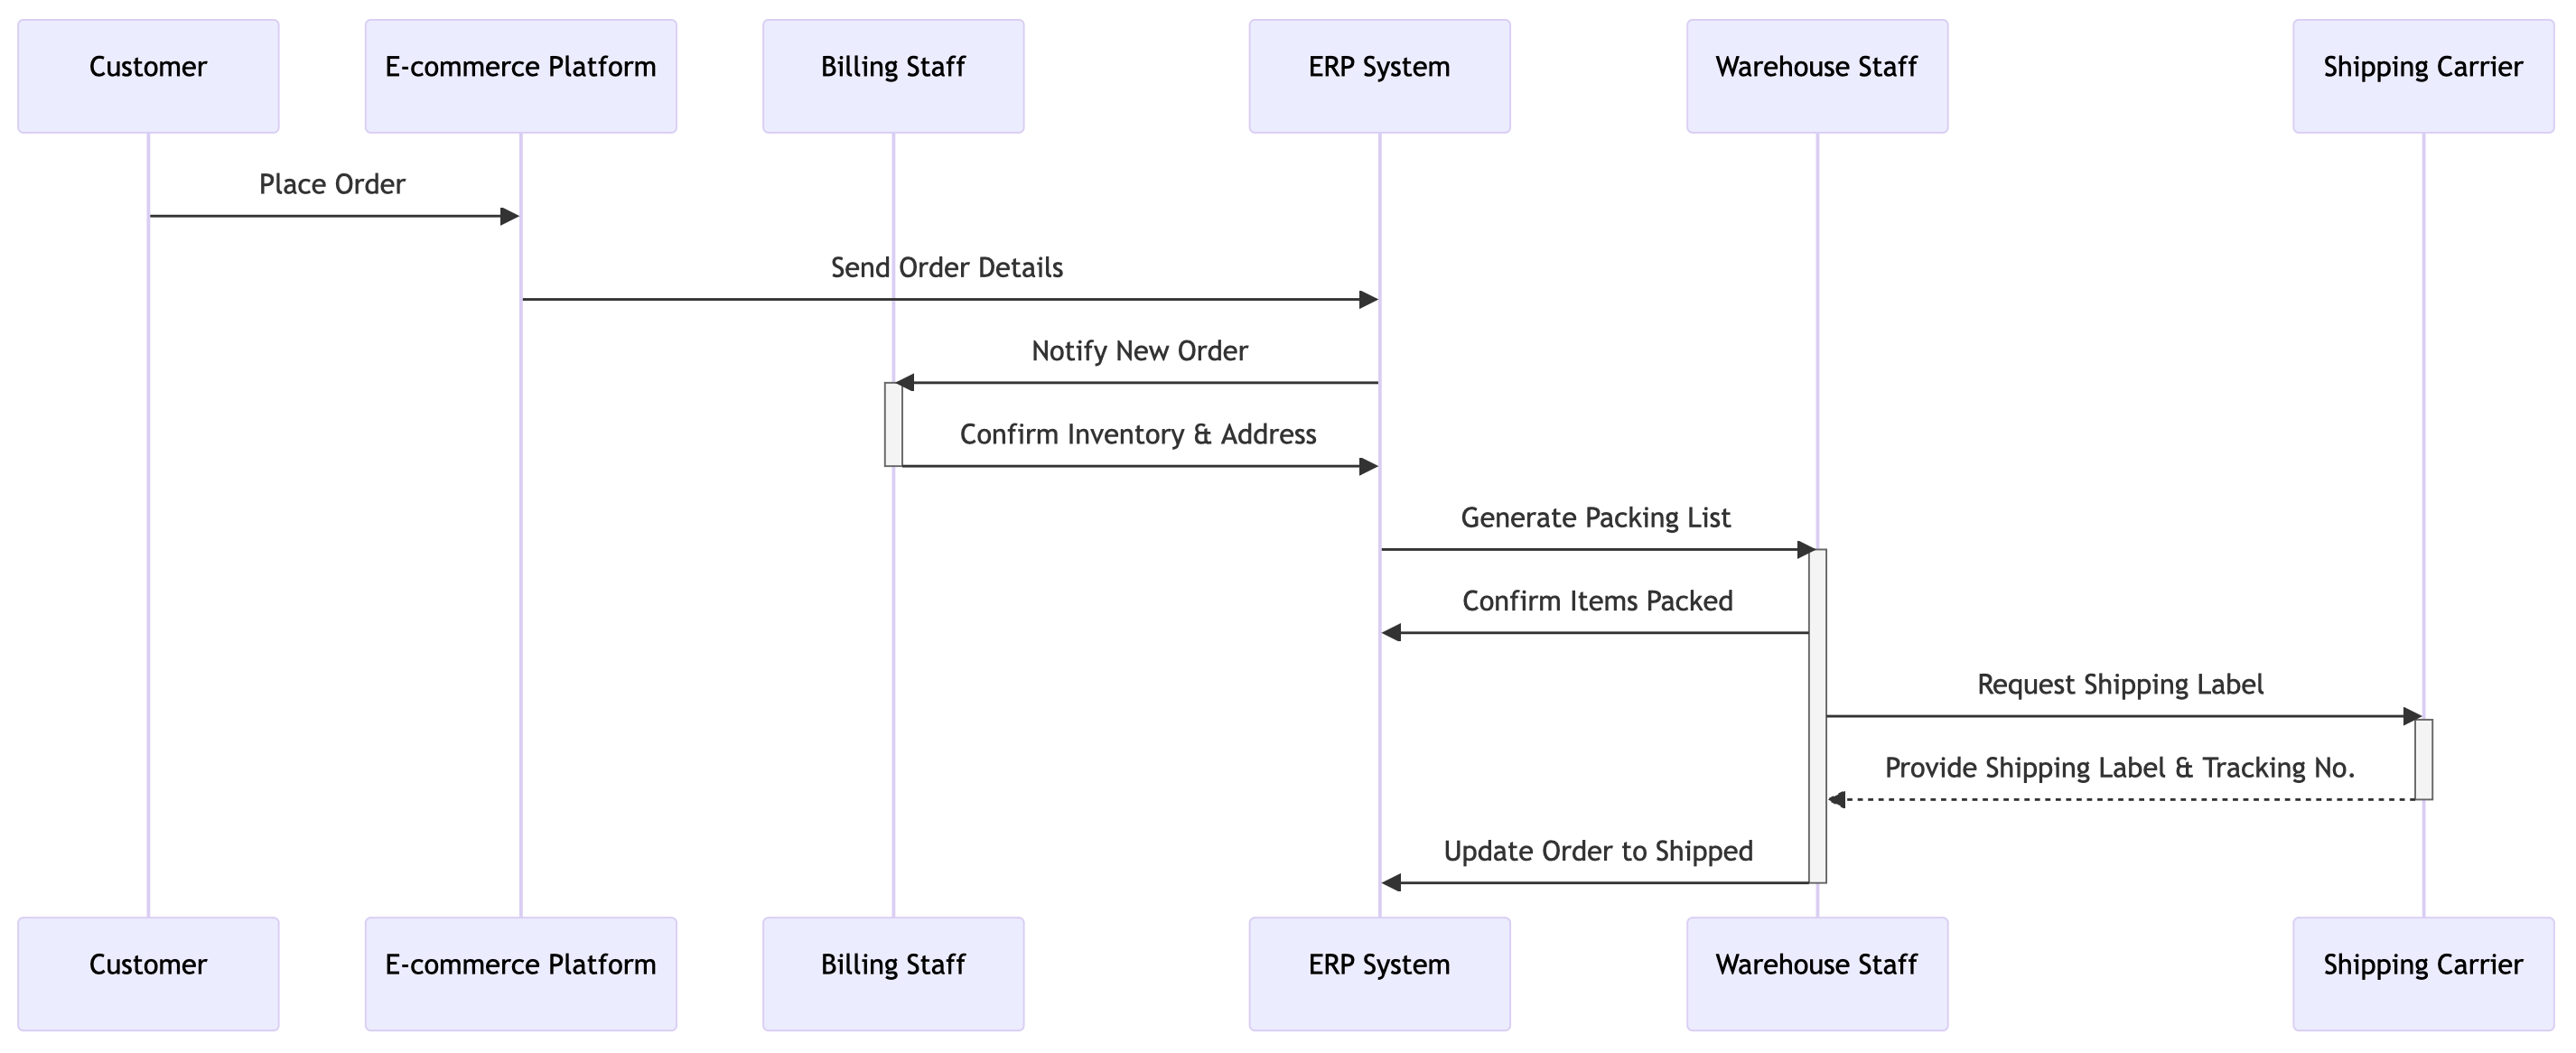
\includegraphics[width=140mm]{img/chap02/fig_proces_sequence_diagram_highres.png}
\caption{Sequence diagram of order dispatching process}
\label{img02:order-dispatch-process}
\end{figure}

%\begin{figure}[H]
%\centerline{\includesvg[width=140mm]{img/chap02/fig_proces_sequence_diagram.svg}}
%\caption{Sequence diagram of order dispatching process}
%\label{img02:order-dispatch-process}
%\end{figure}

\begin{enumerate}
    \item \textbf{Order placement:} Customer completes the checkout process with the shipping details and preferred shipping method. Order information is saved in the e-Commerce platform's database.
    \item \textbf{Order transfer to \ac{ERP}:} The order details are automatically transferred to the \ac{ERP} system. This transfer can occur at scheduled intervals or automatically, depending on the integration setup between the e-Commerce platform and the \ac{ERP}.
    \item \textbf{Order confirmation and inventory check:} The operator of the ERP system in the billing department processes the order with the validation of the shipping address and confirms the order.
    \item \textbf{Packing list and invoice generation:} Once the shipment is confirmed, the \ac{ERP} system generates a packing list that details the items to be shipped. At the same time, an order invoice is created.
    \item \textbf{Uploading shipments data:} With the items collected and packed, the next step involves generating a shipping label. Order data, including recipient information and insurance, are exported from \ac{ERP} to the format accepted by the carrier and uploaded to the carrier interface to retrieve the tracking number for each order.
    \item \textbf{Synchronizing tracking number with \ac{ERP}:} The list of selected orders in \ac{ERP} is altered with the tracking number retrieved from the carrier.
    \item \textbf{Shipping label and consignment list printing:} After orders receive tracking numbers, the shipping labels and the consignment list are downloaded from the carrier interface. The labels are then affixed to the consignments.
    \item \textbf{Shipment dispatch:} Shipments are handed over to the shipping company courier after signing the consignment list as a confirmation of receipt. 
    \item \textbf{Updating status and controlling delivery:} The list of parcel statuses is manually downloaded from the shipping company interface and uploaded to the \ac{ERP} system
\end{enumerate}


After a brief introduction to the process, we can see that points 5-9 are quite challenging.
Since the company may be working with multiple carriers at the same time, we get into a situation where the operator has to repeat these points for each carrier, making the process unsustainable and very time-consuming.
Not to mention that the company has to adapt to each carrier and create data exports and imports for each carrier separately.
In addition, the process of updating shipments is very complex and prone to errors.
For a visualisation using the sequence diagram, refer to \ref{img02:order-dispatch-process}.


% mermaid seq. diagram

%sequenceDiagram
%    participant Customer as Customer
%    participant ECommerce as E-commerce Platform
%    participant Billing as Billing Staff
%    participant ERP as ERP System
%    participant Warehouse as Warehouse Staff
%    participant Shipping as Shipping Carrier

%    Customer->>ECommerce: Place Order
%    ECommerce->>ERP: Send Order Details
%    ERP->>Billing: Notify New Order
%    activate Billing
%    Billing->>ERP: Confirm Inventory & Address
%    deactivate Billing
%    ERP->>Warehouse: Generate Packing List
%    activate Warehouse
%    Warehouse->>ERP: Confirm Items Packed
%    Warehouse->>Shipping: Request Shipping Label
%    activate Shipping
%    Shipping-->>Warehouse: Provide Shipping Label & Tracking No.
%    deactivate Shipping
%    Warehouse->>ERP: Update Order to Shipped
%    deactivate Warehouse



\section{Real-world applicability}
\label{sec:real-world-applicability}
% briefly note that the solution will be integrated and tested in the operating company
% it means for us, that we have to do implementation of three operating shipping carriers in the Czech republic (Ceska Posta, PPL, Packeta) so that company can seamlessly transtion + SAP integrations (so that the data can be stored in SAP for internal purposes and mark orders as shipped).
Platofrm's real-world applicability will be verified through integration and testing within an operating company.
Practical implementation will focus on incorporating three major shipping carriers in the Czech republic - Česká Pošta, PPL, and Packeta - to allow the company to make a seamless transition to use the platform.
This means that the platform will gain three carrier implementations with testing to offer to the rest of the user base.
Together with testing integration capabilities with external systems, namely \gls{sapb1}, it will be necessary to create a connector module presented in chapter \ref{chap:integrating-sap-b1}.

\section{Requirements}
\label{sec:requirements}
% intro, requirements (ref https://engineering.futureuniversity.com/BOOKS%20FOR%20IT/Software-Engineering-9th-Edition-by-Ian-Sommerville.pdf) with descriptiion of what's functional/nonfunctional requirement 
This section introduces the concept of software requirements.
In general, requirements are descriptions of the system's functionalities and what it should do while reflecting the needs of actors.
Requirements can be classified into two groups \cite{sommervilleSW}:
\begin{enumerate}
    \item \textit{Functional requirements:} describes how the system should react to particular inputs and how the system should behave in particular situations.
    \item \textit{Non-functional requirements:} constraints on the services of functions by the system. Including development process constraints and constraints defined by some standards. Non-functional requirements often apply to the system as a whole, rather than individual features.
\end{enumerate}
%For a better description, we will define the three actors used in the requirements later.
The whole system has three expected user roles:
\label{sec:requirements-actors}
\begin{enumerate}
    \item \textbf{Operator:} Role attributed to individuals employed by the company, interacting with the platform through its user interface. 
    \item \textbf{Developer:} Individual in this role utilises the platform's API for developing third-party integration.
    \item \textbf{Customer:} This role represents the end recipients who are waiting for the packages dispatched by the company using the platform.
\end{enumerate}

\begin{figure}[H]\centering
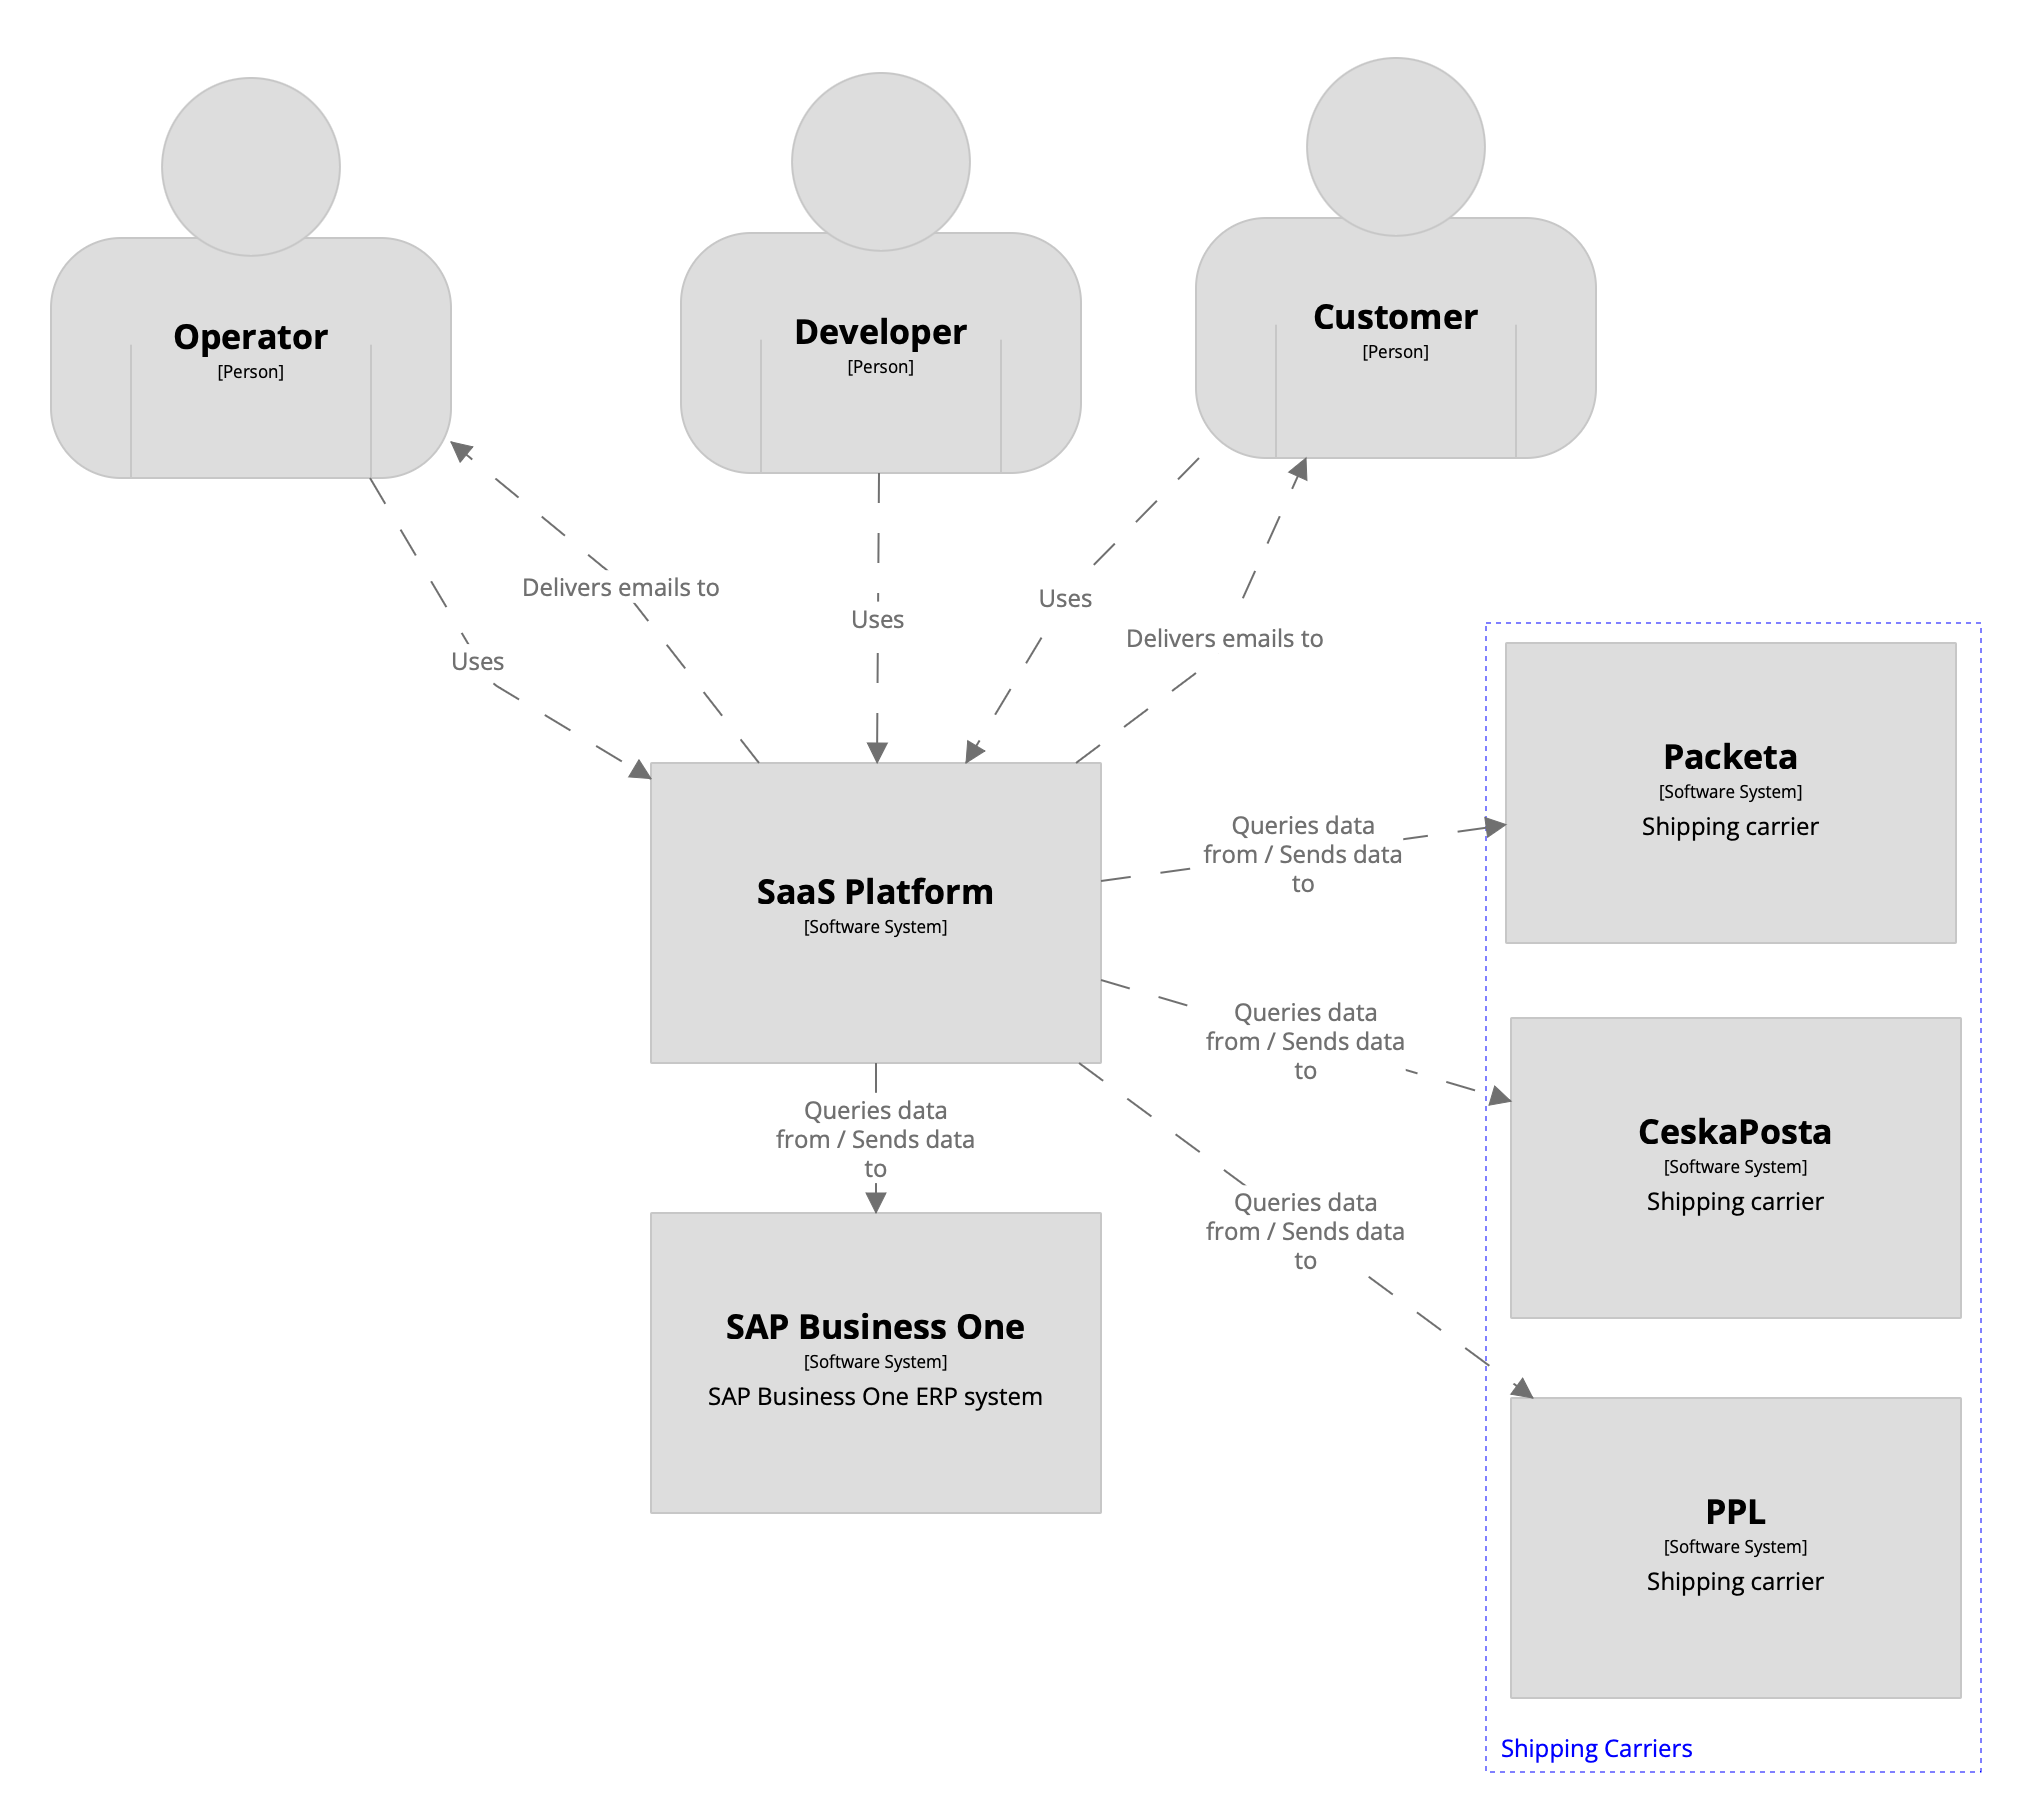
\includegraphics[width=140mm]{img/chap02/fig_system_context.png}
\caption{C4 diagram with system context}
\label{img02:analysis.system-context}
\end{figure}

To provide context, the platform operates as a \ac{SaaS} model and involves three key actors. We will demonstrate integration capabilities using \gls{sapb1}, along with production integration with three carriers: Packeta, PPL, and Česká Pošta. For a visual representation of the system context, refer to Figure \ref{img02:analysis.system-context}.

\subsection{Functional Requirements}
\label{subsec:functional-requirements}
% functions of the software itself and behaviour in given situations

%After researching the related work from chapter \ref{chap:related-work} and looking into the process - see section \ref{sec:order-dispatching-process}, a rough list of requirements was created based on information that can be freely obtained (for example, just from documentation and technical descriptions of existing solutions).
After reviewing the related work presented in Chapter \ref{chap:related-work} and analysing the process detailed in Section \ref{sec:order-dispatching-process}, an initial set of requirements was created.
These were primarily derived from readily available information, such as documentation and technical descriptions of existing solutions.

The whole list was then discussed with the company management (including IT and marketing) where the platform will be deployed for testing; see Section \ref{sec:real-world-applicability}. 
At the same time, the requirements were continuously communicated to the company's warehouse staff, who are considered as \textbf{operators} described in \ref{sec:requirements-actors} and will use the platform to get an overview of the processes and various situations that occur regularly and irregularly.

This newly acquired information provided the opportunity to design the requirements so that it would fit perfectly into the company's daily operations. 
The requirements were then slightly modified according to our own requirements for the platform, such as the limitation to the possibility of using one instance by multiple users, i.e. the platform should be designed as Software as a Service.


%\pointedenum\begin{enumerate}[\bfseries {FR}1{:}]
\begin{enumerate}[label=\bfseries FR\arabic*:,leftmargin=*]
    \item Operators can sign up and verify their accounts using a verification code sent to their provided email address.
    \item Operators can change password to their accounts using a verification code sent to their provided email address.
    \item Operators can log into their accounts using valid credentials.
    \item Operators can switch the interface language between Czech and English.
    \item Operators can create multiple \glspl{project} within their account to manage data separately (e.g., for different warehouses or companies).
    \item Operators can select and work within a specific \gls{project}.
    \item Operators can rename any of their \glspl{project}.
    \item Operators can delete any of their \glspl{project}.
    \item Operators can configure a default shipper for all shipments within a\\ \gls{project}.
    \item Operators can configure settings for shipping carrier APIs, including authentication (e.g., tokens, IDs, secrets) and other required fields.
    \item Within each \gls{project}, operators can create multiple sellers to customise the location and branding of the tracking page and the email notifications.
    \item For each \gls{seller}, operators can set the name, localization, and branding elements such as logo, primary colour, contact information (URL, email, phone, store name), and social media links (Facebook, Instagram,\\ YouTube, TikTok). Operators can also enable customer email notifications for specific parcel statuses.
    \item Operators can remove any \gls{seller} from a \gls{project}.
    \item Operators can enter edit mode of the \gls{seller}.
    \item In \gls{seller} edit mode, operators can switch views between web and email to preview customer-facing pages and emails.
    \item Operators can generate API access tokens for developers to use.
    \item Operators can switch between \glspl{project} to which they have access.
    \item The operator can invite other operators to the \glspl{project}.
    \item Operators can invite new operators to collaborate on \glspl{project}.
    \item \Gls{project} collaborators can be assigned different roles (Owner, Admin, Member) with varying levels of permissions.
    \item Operators can view a paginated list of all shipments.
    \item Operators can adjust the number of shipment items displayed per page.
    \item Operators can navigate through the shipment list pages (next or previous).
    \item Operators can easily identify shipments by carrier (using colour coding and names) and those created on the current day directly from the list.
    \item Operators can apply filters to search through shipments based on textual data (reference, email) using four criteria (equal to, contains, starts with, ends with), date-time data (creation date) using a range picker, and list types (carrier, status) selecting multiple values.
    \item Operators can select multiple shipments across carriers and perform bulk actions on the selected items.
    \item Operators can send shipment data to carriers for all selected bulk shipments.
    \item Operators can generate shipping labels for selected shipments.
    \item Operators can generate a consignment list for selected shipments.
    \item Operators can initiate the creation of a new shipment with a single click on the shipment list page.
    \item When creating a new shipment, operators can specify details such as recipient, insurance, payment method and amount, carrier, and carrier services.
    \item Operators can add multiple parcels to a single shipment.
    \item Operators can preview or delete shipments after they have been sent to the carrier.
    \item Operators can edit or delete shipments before they are sent to the carrier.
    \item The system will automatically update the status of the shipments.
    \item If allowed by the seller, a notification email is sent to the customer when the status of the package is updated.
    \item Developers can retrieve all \gls{project} shipments through the API.
    \item Developers can create or update individual or multiple shipments through the API.
    \item Developers can list all parcels from the \gls{project} via the API.
    \item Developers can retrieve labels for selected shipments through the API.
    \item Developers can initiate the sending of shipment data to carriers for selected shipments via the API.
    \item Customers can receive branded email notifications about updates in the status of the parcel when permitted by the \gls{seller}.
    \item Customers can view the tracking page, customised with the seller's branding, displaying the parcel statuses.
\end{enumerate}

\subsection{Nonfunctional Requirements}
\label{subsec:nonfunctional-requirements}
% quality attributes of the software
% Multi-tenant architecture
% Docs
% CI/CD
% Source code (formatting, conventions)
% support for multiple carriers
The non-functional requirements were shaped by understanding the broader operational context.
These requirements focus on the quality attributes of the platform.

\subsubsection{Usability}
The user interface should be intuitive, requiring minimal training for warehouse and billing staff.
The dashboard of the platform is designed primarily to be used with a mouse and keyboard on standard desktop screens, but should also support touch interactions for versatility.
In addition, the tracking page is optimised primarily for touch interactions on mobile phones to enhance accessibility and ease of use for customers on the go. 
Provide user documentation, including guides for key processes.


\subsubsection{Extensibility}
The system should be able to easily integrate new APIs of the shipping carriers according to user demands.
Any new carrier integration should be seamlessly incorporated into the existing system, ensuring that from a user's perspective, the interaction remains uniform across all carriers.
This means that the user can initiate shipping processes with a single action, regardless of the carrier, allowing the system to handle the specifics in the background.

\subsubsection{Scalability}
Design the system to scale effortlessly to accommodate increases in both user base and request volume. 
The deployment strategy should enable automatic scaling based on current load, ensuring consistent performance even during peak operational periods. 
This approach ensures that the system remains responsive and efficient as demand grows.

%The infrastructure should automatically adjust resources based on load, ensuring seamless performance during peak times.

\subsubsection{Maintainability}
%Use coding standards and best practices to ensure that the source code is clean and easy to maintain.
To ensure that the source code is clean and easy to maintain, we will adhere to recognised coding standards and best practices. 
Specifically, we will use the Airbnb coding standard, which is widely respected for maintaining high-quality code in JavaScript environments.
Furthermore, \gls{eslint} will be employed as a linting tool to automatically check for errors and enforce these standards consistently throughout the development team.
Use a \ac{CI}/\ac{CD} pipeline for simple deployment and minimal downtime. 

\subsubsection{Multi-tenancy}
The system must support a multi-tenant architecture, allowing multiple companies to use the service simultaneously while keeping their data isolated.

\subsubsection{Integration}
Offer an API that supports integration with external systems with clear documentation.
Authentication should be handled by generating a long-lived token.

\subsubsection{Customization}
Allow for easy user customisation, including branded tracking pages and email notifications, to maintain consistency with the brand identity.



